\chapter{Bausteine}

\section{Beispiel für Tabelle}

%Tabelle START
\vspace*{-2.5mm}
\renewcommand{\arraystretch}{1.2}
\begin{table}[h!]
	\centering
	\caption{Abmessungen der Probekörper vor dem Zugversuch}
	\label{tab:tabelle1}
	\begin{tabulary}{\textwidth}{C|CCC}
		\hline
		\textbf{Probe}  &\textbf{Breite [mm]}&\textbf{Dicke [mm]}&\textbf{Anf.-länge[mm]} \\ 
		\hline
		Kupfer (gewalzt) & 12,5 &3,00&50\\
		Kupfer (geglüht) & 12,5&3,00&50\\
		PA6 & 10,0&4,00&50\\
		PP (EPR-30\% Kautschuk) & 9,9 &3,95&50\\
		\hline
	\end{tabulary}
\end{table}
\FloatBarrier
\vspace*{-2.5mm}
%Tabelle ENDE

\section{Beispiel für Skalierbare Tabelle}
\begin{table}[h!]
	\centering
	\resizebox{0.5\textwidth}{!}{
		\begin{tabulary}{\textwidth}{C|C|C|C}
			\textbf{Name} & \textbf{Anwendung}&\textbf{Gleichung}&\textbf{Stoffkonstante} \\ 
			\hline  
			KICK& $x_{80_\omega}>\SI{50}{\milli\meter}$ &$e_{KICK}=c_K*log(\frac{x_{80_\omega}}{x_{80_\alpha}})$&$c_K=1,15*\frac{c_B}{\sqrt{0,05\si{\meter}}} \left[\si{\raiseto{2}\meter\per\raiseto{2}\second}\right]$\\
			BOND&$\SI{50}{\micro\meter}<x_{80_\omega}<\SI{50}{\milli\meter}$&$e_{BOND}=c_B*\left(\frac{1}{\sqrt{x_{80_\omega}}}-\frac{1}{\sqrt{x_{80_\alpha}}}\right)$& $c_B$: tabelliert $\left[\si{\raiseto{2,5}\meter\per\raiseto{2}\second}\right]$\\ 
			RITTER& $x_{80_\omega}>\SI{50}{\micro\meter}$&$e_{RITT}=c_R*\left(\frac{1}{x_{80_\omega}}-\frac{1}{x_{80_\alpha}}\right)$&$c_R= 0,5*c_B*\sqrt{\SI{5e-5}{\meter}}$ \\  
	\end{tabulary}}
\end{table}
\FloatBarrier

\section{Tabelle mit Itemize}
%Tabelle START
\vspace*{-2.5mm}
\renewcommand{\arraystretch}{1.2}
\begin{table}[h!]
	\centering
	\caption{Vor- und Nachteile der Geothermie}
	\label{tab:tabelle1}
	\begin{tabulary}{\textwidth}{C|C}
		\hline
		\textbf{Vorteile}  &\textbf{Nachteile} \\ 
		\hline
		&\\
		\begin{minipage}[t]{0.4\textwidth}
			\begin{itemize}
				\item Strom, Wärme und Kälte wird erzeugt
				\item keine saisonalen und tageszeitlichen Schwankungen
				\item 	quasi-regenerativ
				\item 	nachfrage-gerechte Energiebereitstellung
			\end{itemize}
		\end{minipage} & 
		\begin{minipage}[t]{0.4\textwidth}
			\begin{itemize}
				\item hohe Anschaffungskosten
				\item abhängig von geologischen Gegebenheiten
				\item geringer Stromwirkungsgrad (thermodynamisch bedingt)
				\item keine Marktdurchdringung in DE
			\end{itemize}
		\end{minipage}\\
	\end{tabulary}
\end{table}
\FloatBarrier
\vspace*{-2.5mm}
%Tabelle ENDE

\section{Beispiel für Berechnungen}
Die Berechnung der wahren Spannung $\sigma_{W}$ bei Höchstkraft erfolgt unter der Annahme, dass der Prüfkörperquerschnitt noch 60\% des Ausgangsquerschnitts beträgt. Die Berechnung erfolgt ab Gleichung \ref{ber1}. 

%Start
\begin{flalign}
\label{ber1}
\text{\textbf{Endquerschnitt} } \boldsymbol{S_{End}} \text{\textbf{:}} &&	S_{End} = S_{0_{Kupfer (weich)}}*0,6 &&
\end{flalign}
\begin{flalign}
\hspace*{9em} 	&& S_{End} 	&= 37,5mm^2*0,6 && \\
&&			&=\underline{22,5mm^2}&&
\end{flalign}
%Ende

%Start
\begin{flalign}
\text{\textbf{Maximale Kraft}} \boldsymbol{F_{max}} \text{\textbf{:}} && F_{max}=R_{m}*S_{0_{Kupfer (weich)}} &&
\end{flalign}
\begin{flalign}
\hspace*{12em} &&	F_{max}	&=232\frac{N}{mm^2}*37,5mm^2 &&\\
&&			&=\underline{\underline{8700N}} &&
\end{flalign}
%Ende

\newpage

\section{Beispiel für ein Bild}

%Start
\begin{figure}[h!]
	\centering
	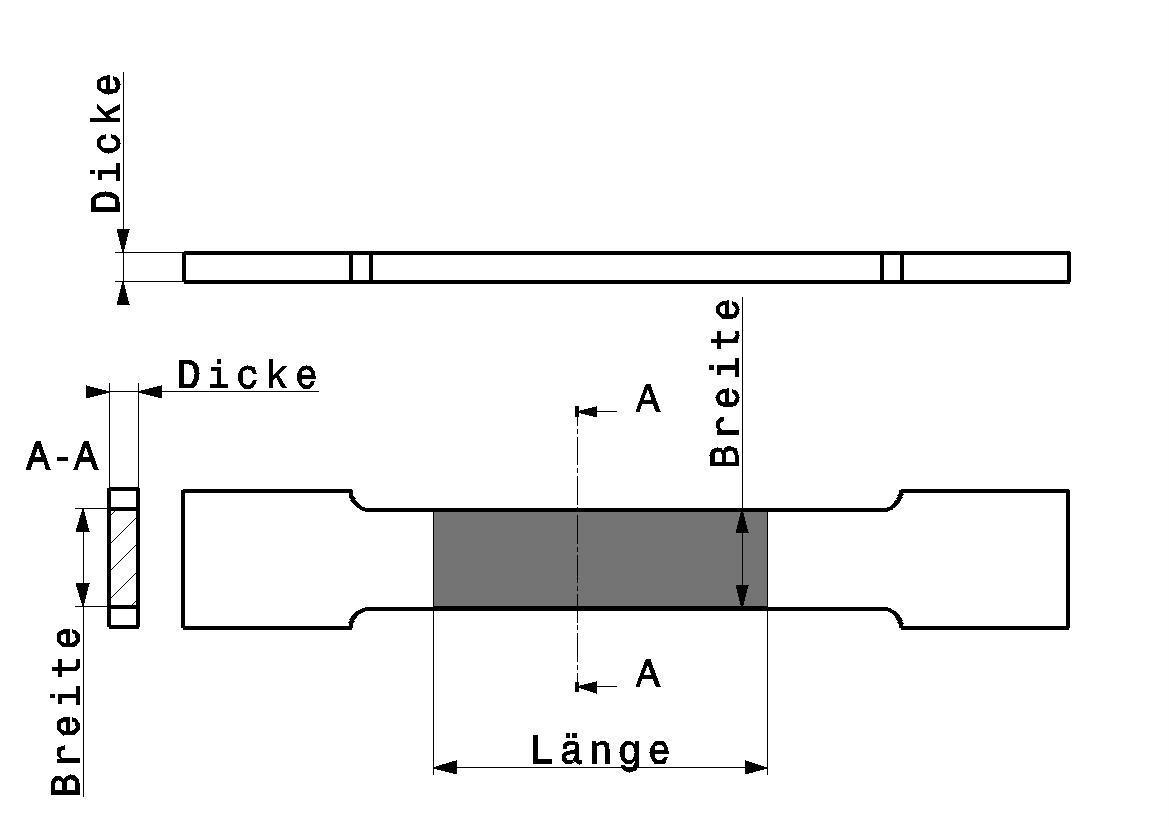
\includegraphics[width=0.60\textwidth]{img/skizzepruef3}
	\caption{Skizze Prüfkörperbemaßung}
	\label{skizzepruef}
\end{figure}
\FloatBarrier
%Ende

\section{Beispiel für zwei Bilder}
\label{sec:versuchsaufbau}

%Start
\begin{figure}[h!]
	\centering
	\begin{subfigure}{.5\textwidth}
		\centering
		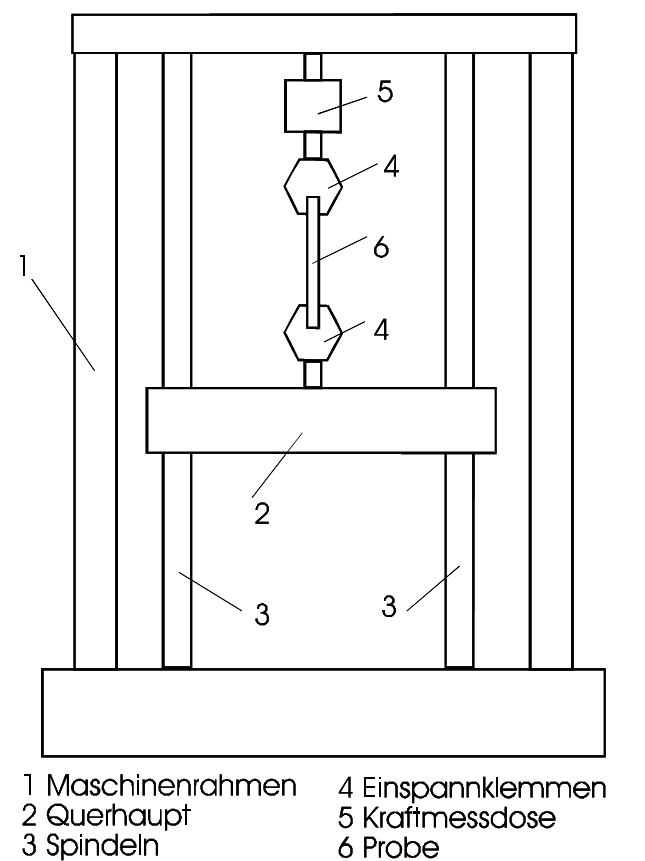
\includegraphics[width=0.75\textwidth]{img/Aufbau2}
		\caption{Skizze zum Versuchsaufbau}
		\label{fig:sub1}
	\end{subfigure}%
	\begin{subfigure}{.5\textwidth}
		\centering
		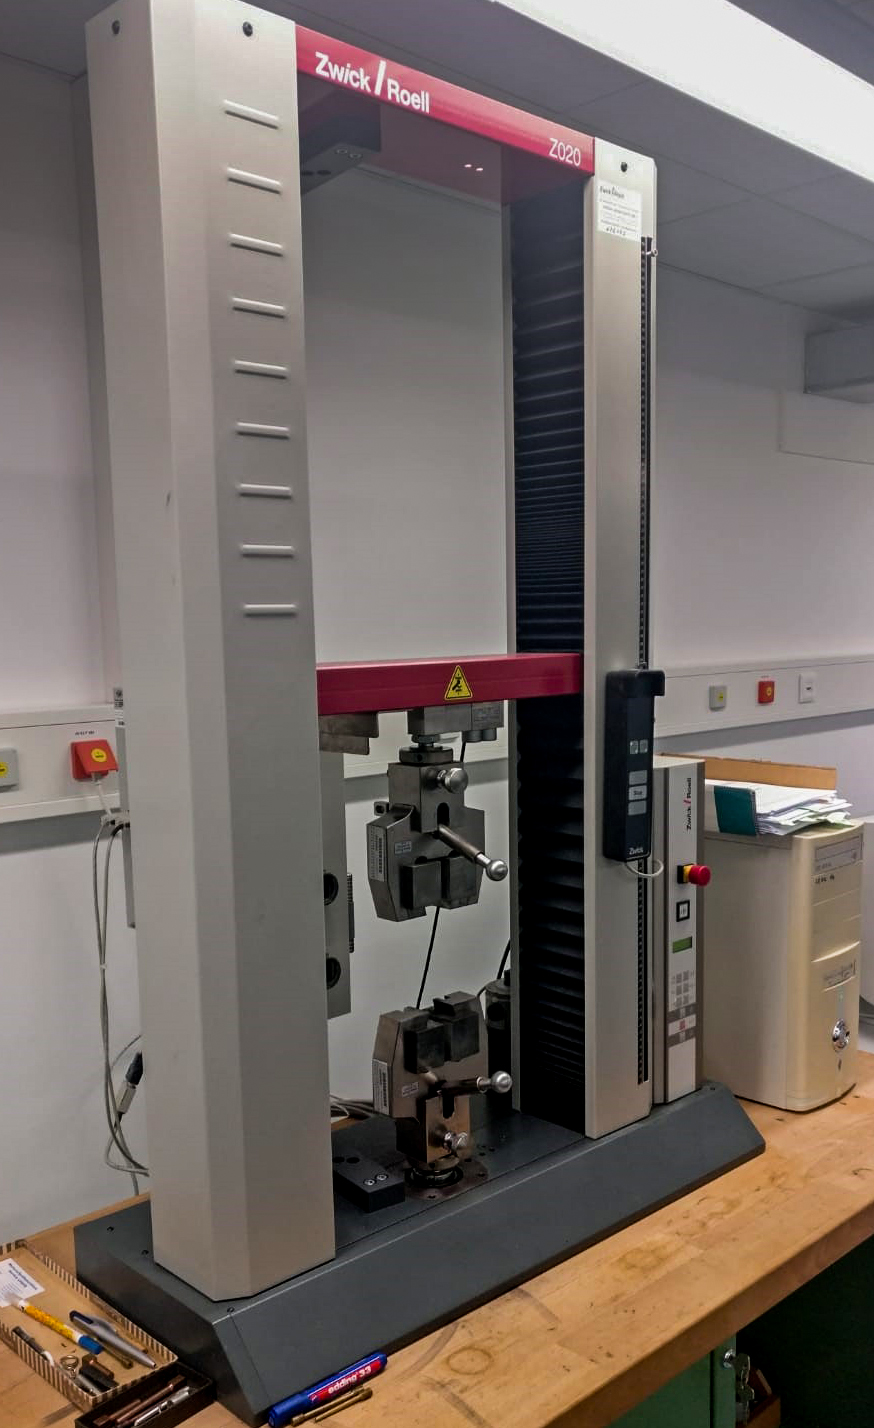
\includegraphics[width=0.6\textwidth]{img/Aufbau1}
		\caption{realer Versuchsaufbau}
		\label{fig:sub2}
	\end{subfigure}
	\caption{Versuchsaufbau als Skizze und in Realität}
	\label{fig:aufbau} 
\end{figure}
\FloatBarrier
%Ende

\newpage


\section{Beispiel für vier Bilder}
%Start
\begin{figure}[h!]
	\centering
	\begin{subfigure}{.5\textwidth}
		\centering
		\includegraphics[width=0.75\textwidth]{img/Kupfer_gewalzt}
		\caption{Kupfer (gewalzt)}
		\label{fig:sub3}
	\end{subfigure}%
	\begin{subfigure}{.5\textwidth}
		\centering
		\includegraphics[width=0.75\textwidth]{img/Kupfer_weich}
		\caption{Kupfer (geglüht)}
		\label{fig:sub4}
	\end{subfigure}
	\begin{subfigure}{.5\textwidth}
		\centering
		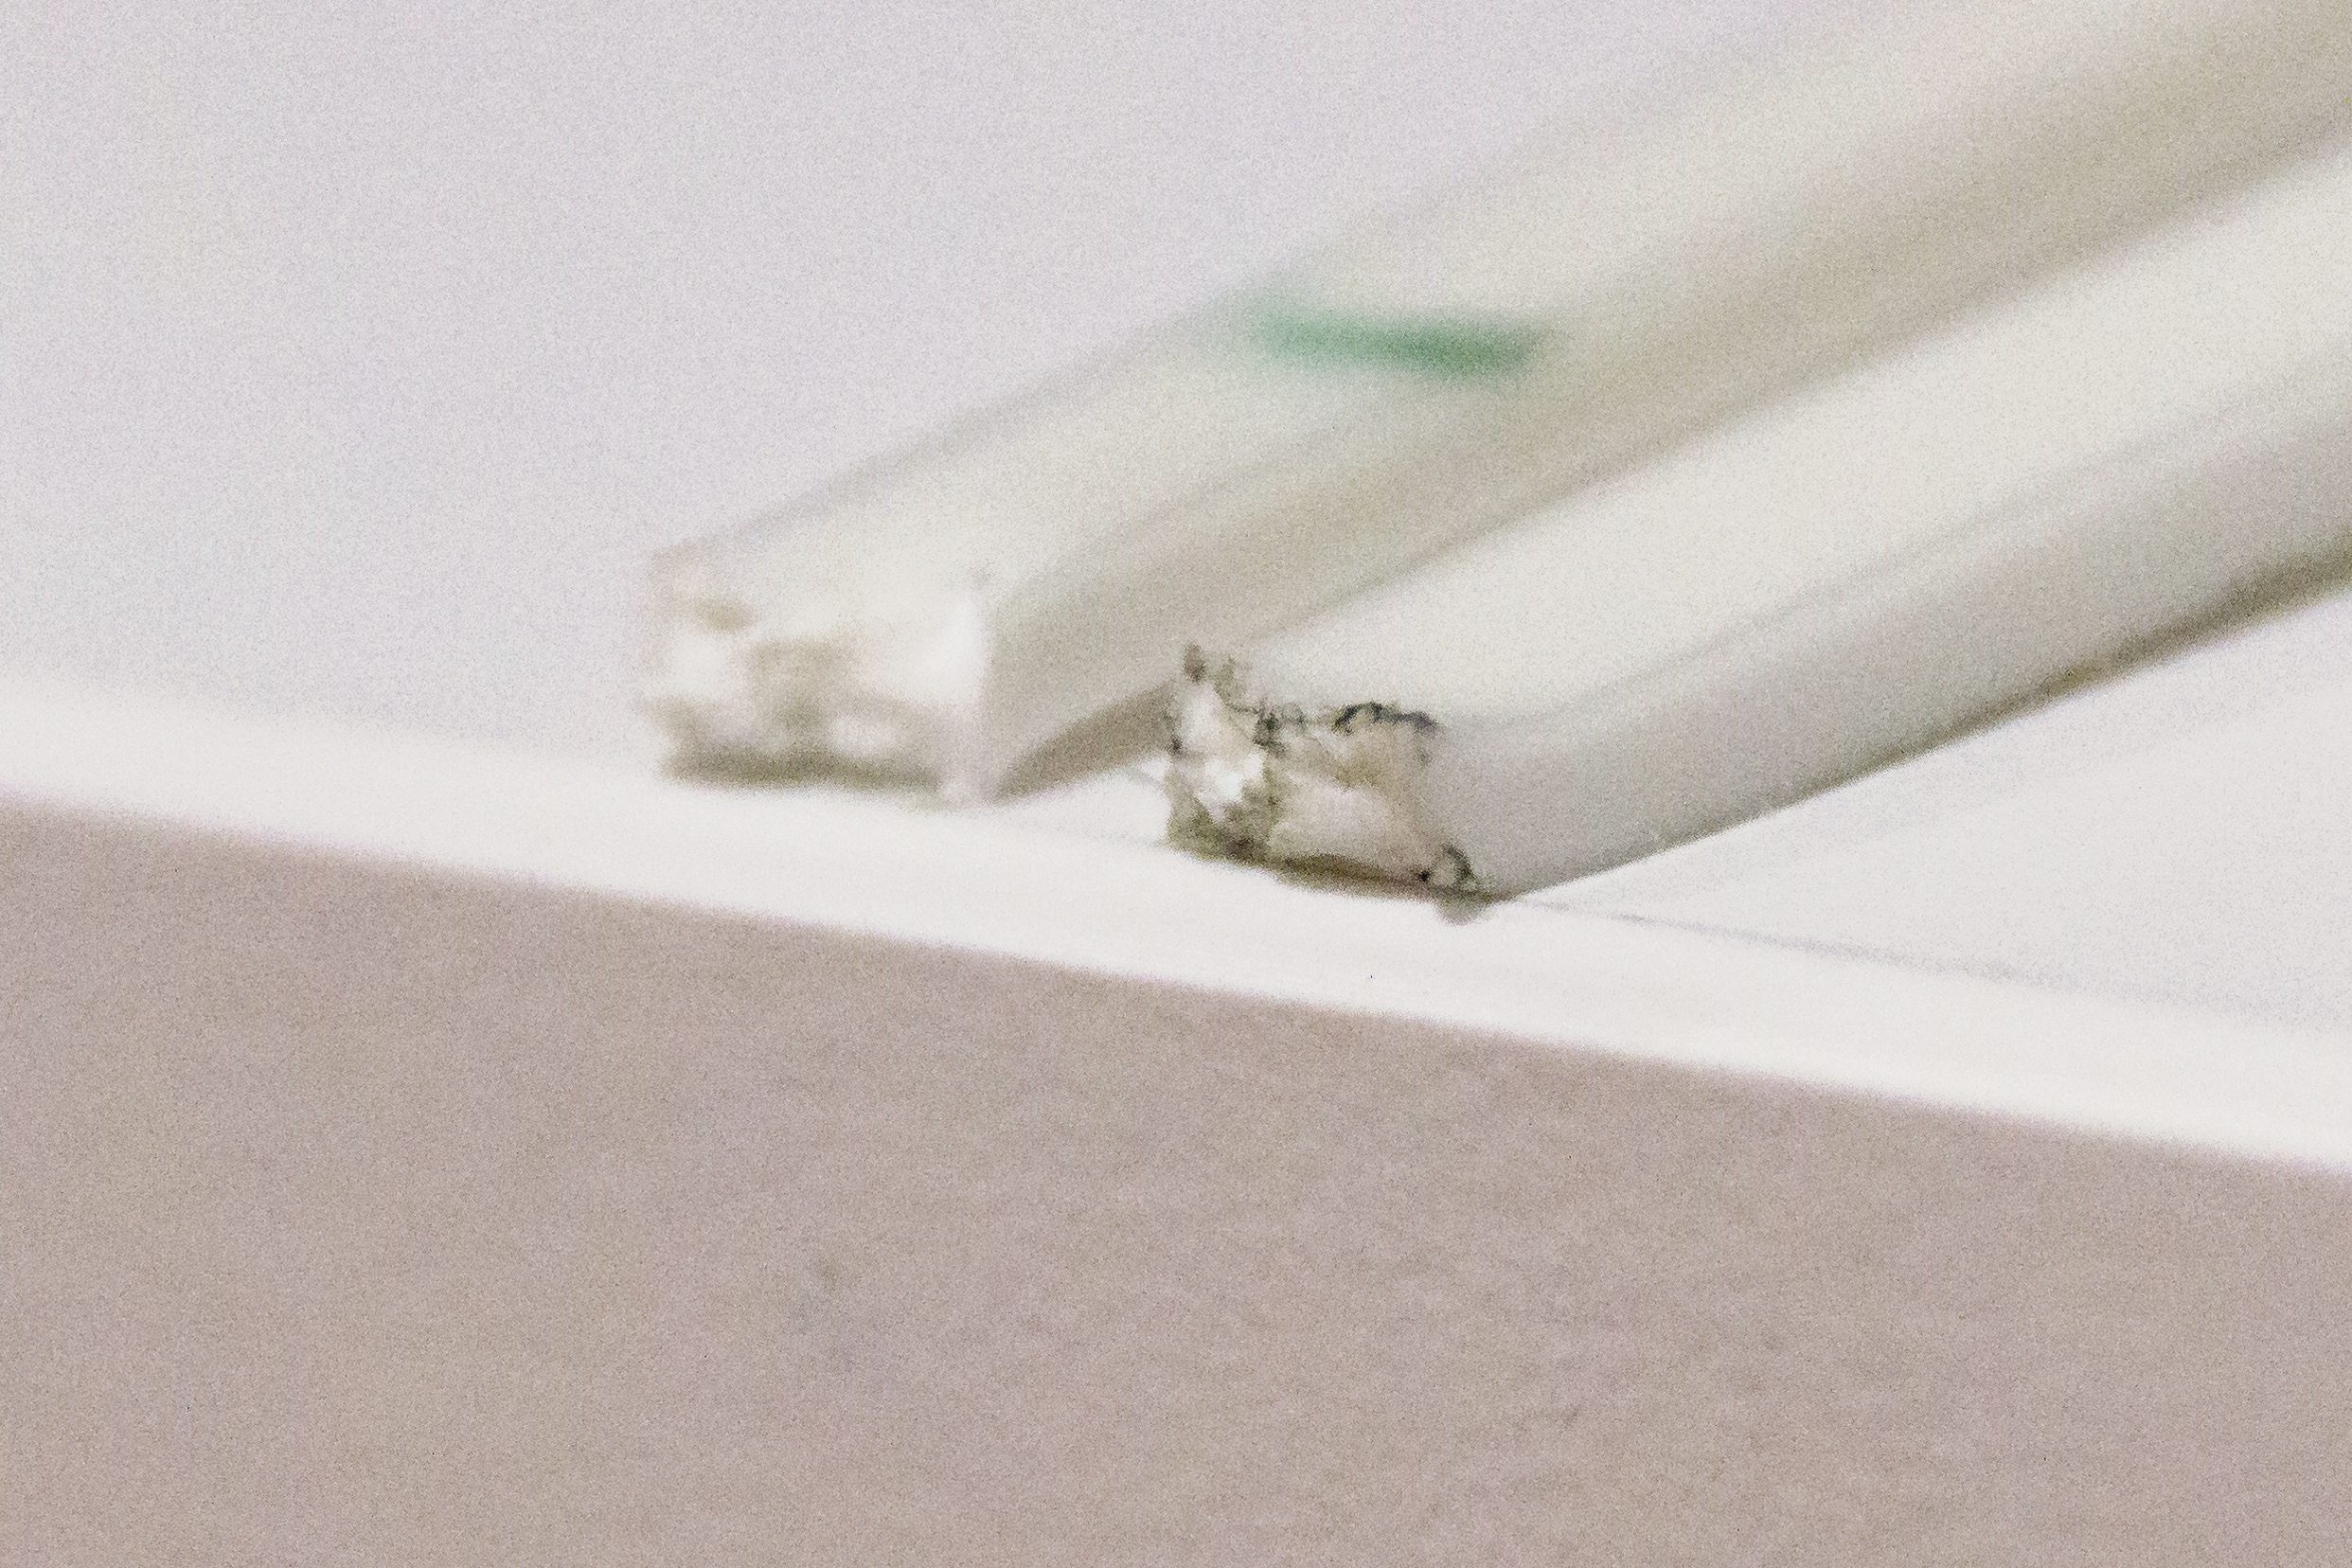
\includegraphics[width=0.75\textwidth]{img/PA6}
		\caption{PA6}
		\label{fig:sub5}
	\end{subfigure}%
	\begin{subfigure}{.5\textwidth}
		\centering
		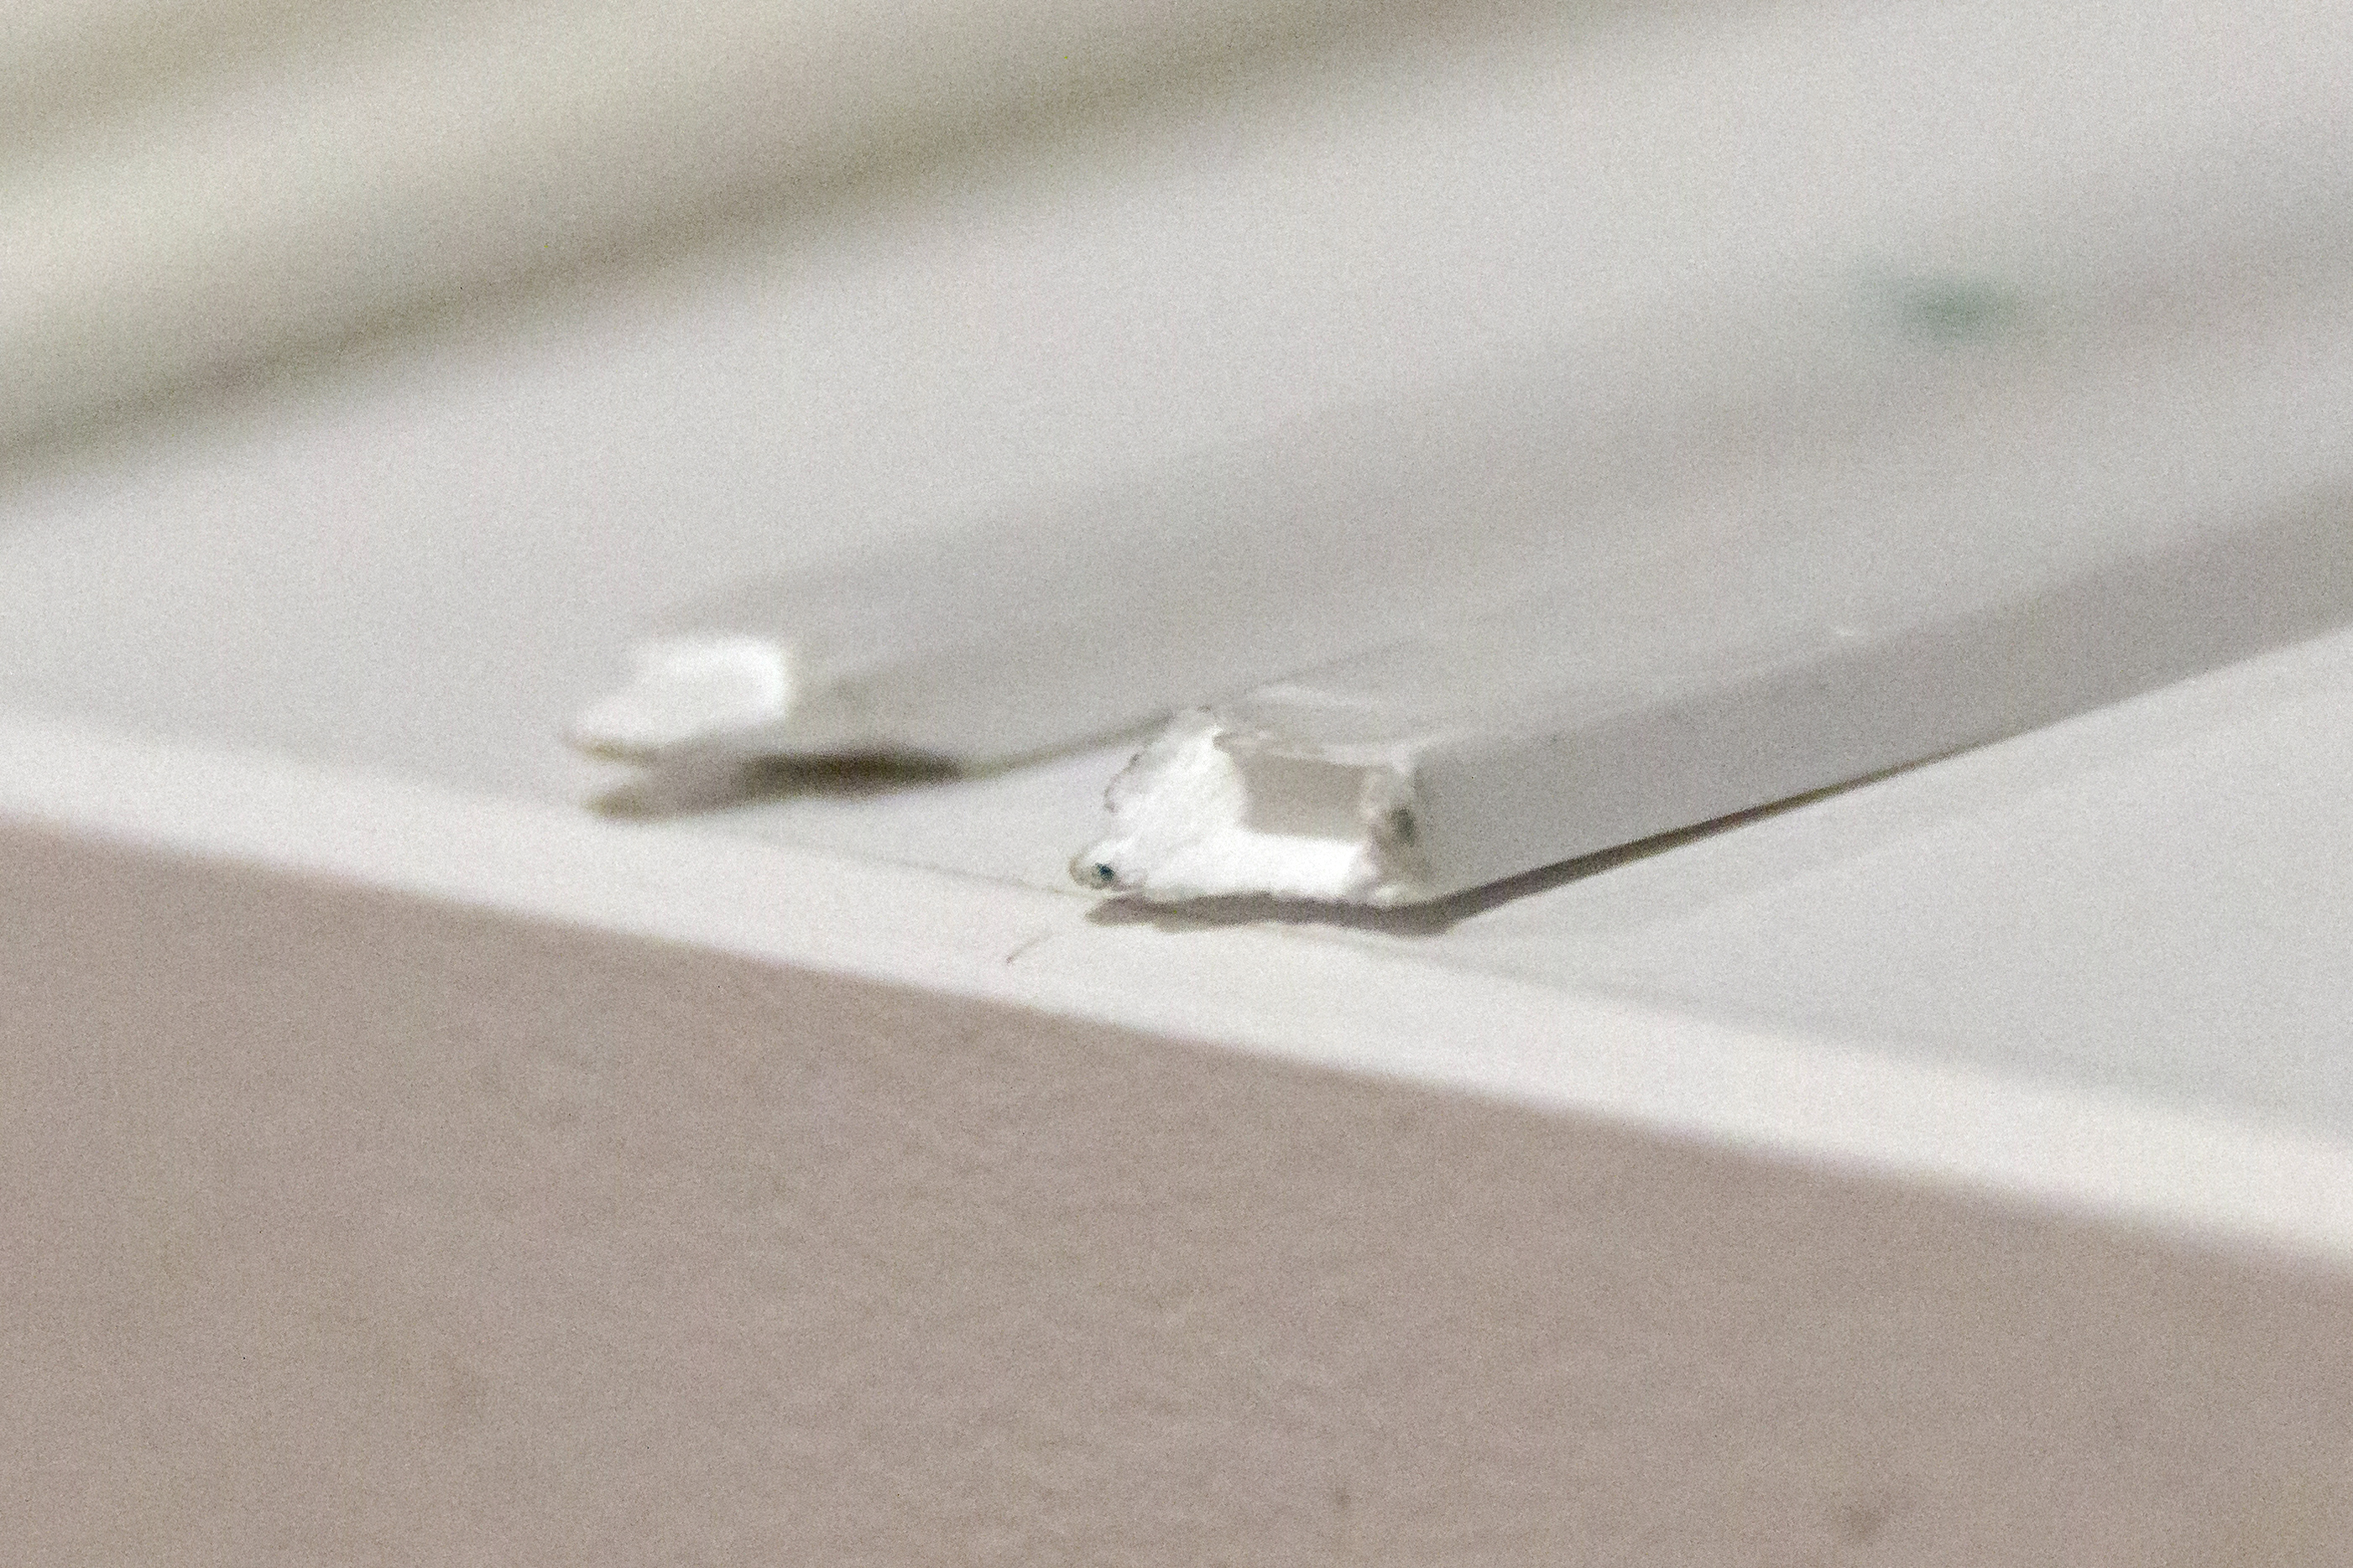
\includegraphics[width=0.75\textwidth]{img/PP}
		\caption{PP (ERP-30\% Kautschuk)}
		\label{fig:sub6}
	\end{subfigure}
	
	\caption{Bruchstellennahaufnahmen der Probekörper}
	\label{fig:bruchstellen} 
\end{figure}
\FloatBarrier
%Ende

\section{Beispiel Einheiten}

\begin{align*}
\textbf{$\SI{12,0/12}{\kg\meter\per\second \raiseto{5} \per \xyz}*\SI{13}{\per\raiseto{-2}\meter}=\SI{256}{}$}
\end{align*}

\begin{align}
\SI{12,0/12}{\meter\per\joule}*\SI{13}{\gram}=\SI{256}{\coulomb}
\end{align}

\newpage

\section{Beispiel für Mini-Formelsammlung}
\begin{flalign}
\label{gl1}
\text{\textbf{Dehnung (Def.)} } \boldsymbol{\varepsilon} \text{ \textbf{:}} && \hspace*{-1em}  \varepsilon=\frac{\Delta l}{l_0} &&
\end{flalign}

\begin{flalign}
\label{gl2}
\text{\textbf{norminelle Spannung} } \boldsymbol{\sigma} \text{\textbf{:}} && \hspace*{-3em} \sigma=\frac{F}{A_0} &&
\end{flalign}

\begin{flalign}
\label{gl3}
\text{\textbf{Sekantenmodul (Kunststoffe) }} \boldsymbol{E_S} \text{ \textbf{:}} && E_S=\frac{\sigma_2-\sigma_1}{\varepsilon_2-\varepsilon_1}=\frac{F_2-F_1}{0,002*A_0} &&
\end{flalign}

\begin{flalign}
\label{gl4}
\text{\textbf{E-Modul (Metalle) }} \boldsymbol{E_M} \text{ \textbf{:}} && \hspace*{5em} E_M=\frac{\sigma}{\varepsilon}=\frac{\sigma_2-\sigma_1}{\varepsilon_2-\varepsilon_1}=\frac{R_{p_{0.2\%}}}{0,2\%} &&
\end{flalign}

\begin{flalign}
\label{gl5}
\text{\textbf{Bruchdehnung} } \boldsymbol{A} \text{\textbf{:}} && \hspace*{6em} A= \frac{l_{u}-l_{0}}{l_{0}}*100\% &&
\end{flalign}

\begin{flalign}
\label{gl6}
\text{\textbf{Ausgangsquerschnitt } } \boldsymbol{S_0} \text{\textbf{:}} && \hspace*{3em} S_{0}= Breite*Dicke &&
\end{flalign}
\begin{flalign}
\label{gl7}
\text{\textbf{wahre Spannung} } \boldsymbol{\sigma_{W}} \text{\textbf{:}} &&\hspace*{1em} \sigma_{W}=\frac{F_{max}}{S_{End}}&&
\end{flalign}
\begin{flalign}
\label{gl8}
\text{\textbf{Brucheinschnürung } } \boldsymbol{Z} \text{\textbf{:}} && \hspace*{5em} Z=\frac{S_0-S_u}{S_{o}}*100\% &&
\end{flalign}